\documentclass[11pt, oneside]{article}
\usepackage[letterpaper, margin=2cm]{geometry}
\usepackage{MATH565}

\begin{document}
\noindent \textbf{\Large{Caleb Logemann \\
MATH 565 Continuous Optimization \\
Midterm Exam
}}

%\lstinputlisting[language=Python]{H01_23.m}
\begin{enumerate}
  \item % #1 Done
    \begin{enumerate}
      \item[(a)] % Done
        Derive an expression for the gradient $\v{\nabla f}$.

        In order to derive an expression for $\v{\nabla f}$ we must compute all
        the partial derivatives $\pd{f}{x_k}$ and $\pd{f}{y_k}$ for all
        $1 \le k \le N$.

        In order to compute these partial derivatives, I will first rewrite $f$
        in a way that seperates the $x_k$ and $y_k$ terms.
        \begin{align*}
          f(\v{x}) = \p{(x_k - x_k)^2 + (y_k - y_k)^2 - d_{kk}^2}^2
          + \sum*{\substack{j = 1 \\ j \neq k}}{N}{\p{(x_k - x_j)^2 + (y_k - y_j)^2 - d_{kj}^2}^2} \\
          + \sum*{\substack{i = 1 \\ i \neq k}}{N}{\p{(x_i - x_k)^2 + (y_i - y_k)^2 - d_{ik}^2}^2}
          + \sum*{\substack{j = 1 \\ j \neq k}}{N}{\sum*{\substack{i = 1 \\ i \neq k}}{N}{\p{(x_i - x_j)^2 + (y_i - y_j)^2 - d_{ik}^2}^2}}
        \end{align*}
        By noting that $(x_i - x_k)^2 = (x_k - x_i)^2$ and that $d_{ik} = d_{ki}$,
        this can be simplified to
        \begin{align*}
          f(\v{x}) = d_{kk}^4
          + 2\sum*{\substack{j = 1 \\ j \neq k}}{N}{\p{(x_k - x_j)^2 + (y_k - y_j)^2 - d_{kj}^2}^2}
          + \sum*{\substack{j = 1 \\ j \neq k}}{N}{\sum*{\substack{i = 1 \\ i \neq k}}{N}{\p{(x_i - x_j)^2 + (y_i - y_j)^2 - d_{ik}^2}^2}}.
        \end{align*}
        Now the partial derivatives of this can be taken easily note that the
        first and last terms don't contain $x_k$ or $y_k$.
        The partial derivatives are
        \begin{align*}
          \pd{f}{x_k} &= 8 \sum{\substack{j = 1 \\ j \neq k}}{N}{\p{(x_k - x_j)^2 + (y_k - y_j)^2 - d_{kj}^2}(x_k - x_j)} \\
          \pd{f}{y_k} &= 8 \sum{\substack{j = 1 \\ j \neq k}}{N}{\p{(x_k - x_j)^2 + (y_k - y_j)^2 - d_{kj}^2}(y_k - y_j)}
        \end{align*}
        When $j = k$ the terms of these sums are zero, so these can also be expressed as
        \begin{align*}
          \pd{f}{x_k} &= 8 \sum{j = 1}{N}{\p{(x_k - x_j)^2 + (y_k - y_j)^2 - d_{kj}^2}(x_k - x_j)} \\
          \pd{f}{y_k} &= 8 \sum{j = 1}{N}{\p{(x_k - x_j)^2 + (y_k - y_j)^2 - d_{kj}^2}(y_k - y_j)}.
        \end{align*}

        Now the gradient of $f$ can be written using these partial derivatives, as follows
        \[
          \v{\nabla f}(\v{x}) =
          \begin{bmatrix}
            \pd{f}{x_1} \\
            \pd{f}{y_1} \\
            \pd{f}{x_2} \\
            \pd{f}{y_2} \\
            \vdots \\
            \pd{f}{x_N} \\
            \pd{f}{y_N} \\
          \end{bmatrix}
        \]

      \item[(b)] % Done
        Derive an expression for the Hessian $\M{\nabla^2 f}$.

        The Hessian for this function requires finding all possible partial
        second derivatives.
        There are several possible different partial second derivatives.
        They are $\pd[2]{f}{x_k}$, $\pd[2]{f}{y_k}$,
        $\mpd[2]{f}{\partial x_k \partial y_k}$,
        $\mpd[2]{f}{\partial x_k \partial x_i}$,
        $\mpd[2]{f}{\partial y_k \partial y_i}$, and 
        $\mpd[2]{f}{\partial x_k \partial y_i}$, where $k \neq i$.

        First I will compute $\pd[2]{f}{x_k}$ and $\pd[2]{f}{y_k}$.
        \begin{align*}
          \pd[2]{f}{x_k} &= \pda{8 \sum*{j = 1}{N}{\p{(x_k - x_j)^2 + (y_k - y_j)^2 - d_{kj}^2}(x_k - x_j)}}{x_k} \\
          &= \pda{8 \sum*{j = 1}{N}{(x_k - x_j)^3 + \p{(y_k - y_j)^2 - d_{kj}^2}(x_k - x_j)}}{x_k} \\
          &= 8 \sum*{j = 1}{N}{\pda{(x_k - x_j)^3}{x_k} + \p{(y_k - y_j)^2 - d_{kj}^2}\pda{(x_k - x_j)}{x_k}} \\
          &= 8 \sum*{j = 1}{N}{3(x_k - x_j)^2 + (y_k - y_j)^2 - d_{kj}^2} \\
          \pd[2]{f}{y_k} &= \pda{8 \sum*{j = 1}{N}{\p{(x_k - x_j)^2 + (y_k - y_j)^2 - d_{kj}^2}(y_k - y_j)}}{y_k} \\
          &= 8 \sum*{j = 1}{N}{(x_k - x_j)^2 + 3(y_k - y_j)^2 - d_{kj}^2}
        \end{align*}

        Next I will compute $\mpd[2]{f}{\partial x_k \partial y_k}$.
        \begin{align*}
          \mpd[2]{f}{\partial x_k \partial y_k} &= \pda{8 \sum*{j = 1}{N}{\p{(x_k - x_j)^2 + (y_k - y_j)^2 - d_{kj}^2}(x_k - x_j)}}{y_k} \\
          &= 8 \sum*{j = 1}{N}{(x_k - x_j)\pda{(y_k - y_j)^2}{y_k}} \\
          &= 16 \sum*{j = 1}{N}{(x_k - x_j)(y_k - y_j)}
        \end{align*}

        Thirdly I will compute $\mpd[2]{f}{\partial x_k \partial x_i}$ and
        $\mpd[2]{f}{\partial y_k \partial y_i}$, for $i \neq k$.
        \begin{align*}
          \mpd[2]{f}{\partial x_k \partial x_i} &= \pda{8 \sum*{j = 1}{N}{\p{(x_k - x_j)^2 + (y_k - y_j)^2 - d_{kj}^2}(x_k - x_j)}}{x_i} \\
          &= \pda{8\p{(x_k - x_i)^2 + (y_k - y_i)^2 - d_{ki}^2}(x_k - x_i)}{x_i} \\
          &= \pda{8(x_k - x_i)^3 +8\p{(y_k - y_i)^2 - d_{ki}^2}(x_k - x_i)}{x_i} \\
          &= -24(x_k - x_i)^2 - 8\p{(y_k - y_i)^2 - d_{ki}^2} \\
          &= -8\p{(x_k - x_i)^2 + (y_k - y_i)^2 - d_{ki}^2} \\
          \mpd[2]{f}{\partial y_k \partial y_i} &= \pda{8 \sum*{j = 1}{N}{\p{(x_k - x_j)^2 + (y_k - y_j)^2 - d_{kj}^2}(y_k - y_j)}}{y_i} \\
          &= \pda{8 \p{(x_k - x_i)^2 + (y_k - y_i)^2 - d_{ki}^2}(y_k - y_i)}{y_i} \\
          &= \pda{8 \p{(x_k - x_i)^2 - d_{ki}^2}(y_k - y_i)+ (y_k - y_i)^3}{y_i} \\
          &= -8 \p{(x_k - x_i)^2 + 3(y_k - y_i)^2 - d_{ki}^2}
        \end{align*}

        Lastly I will compute $\mpd[2]{f}{\partial x_k \partial y_i}$ for
        $i \neq k$.
        Note that this is equivalent to $\mpd[2]{f}{\partial y_i \partial x_k}$.
        \begin{align*}
          \mpd[2]{f}{\partial x_k \partial y_i} &= \pda{8 \sum*{j = 1}{N}{\p{(x_k - x_j)^2 + (y_k - y_j)^2 - d_{kj}^2}(x_k - x_j)}}{y_i} \\
          &= \pda{8 \p{(x_k - x_i)^2 + (y_k - y_i)^2 - d_{ki}^2}(x_k - x_i)}{y_i} \\
          &= -16(x_k - x_i)(y_k - y_i)
        \end{align*}

        Now with all these partial derivatives the Hessian can be shown as a
        matrix of partial derivatives.
        \begin{align*}
          \M{\nabla^2 f} =
          \begin{bmatrix}
            \pd[2]{f}{x_1} & \mpd[2]{f}{\partial x_1 \partial y_1} & \cdots & \mpd[2]{f}{\partial x_1 \partial x_N} & \mpd[2]{f}{\partial x_1 \partial y_N} \\
            \mpd[2]{f}{\partial y_1 \partial x_1} & \pd[2]{f}{y_1} & \cdots & \mpd[2]{f}{\partial y_1 \partial x_N} & \mpd[2]{f}{\partial y_1 \partial y_N} \\
            \vdots & \vdots & \ddots & \vdots & \vdots \\
            \mpd[2]{f}{\partial x_N \partial x_1} & \mpd[2]{f}{\partial x_N \partial y_1} & \cdots &  \pd[2]{f}{x_N} & \mpd[2]{f}{\partial x_N \partial y_N} \\
            \mpd[2]{f}{\partial y_N \partial x_1} & \mpd[2]{f}{\partial y_N \partial y_1} & \cdots &  \mpd[2]{f}{\partial y_N \partial x_N} & \pd[2]{f}{y_N} \\
          \end{bmatrix}
        \end{align*}

      \item[(c)] % Done
        Prove that the Hessian, $\M{\nabla^2 f}$ is symmetric positive definite
        for all $\v{x} \in \RR^{2N}$.

        \begin{proof}
          Cleary the Hessian is symmetric as all of the partial derivatives
          are symmetric.
          I don't believe that the Hessian is in face positive definite
          or positive semidefinite.
          In order to show this consider the situation with $N = 2$ that is only
          two cities.
          In this case the $f$ can be written as
          \[
            f(\v{x}) = 2((x_1 - x_2)^2 + (y_1 - y_2)^2 - d_{12}^2)^2
          \]
          I will evaluate the Hessian at $\v{x} = \br{0, 0, 0, 0}^T$.
          In this case the partial derivatives become
          \begin{align*}
            \pd[2]{f}{x_k} &= 8 \sum*{j = 1}{2}{3(x_k - x_j)^2 + (y_k - y_j)^2 - d_{kj}^2} \\
            &= -8d_{12}^2 \\
            \pd[2]{f}{y_k} &= 8 \sum*{j = 1}{2}{(x_k - x_j)^2 + 3(y_k - y_j)^2 - d_{kj}^2} \\
            &= -8d_{12}^2 \\
            \mpd[2]{f}{\partial x_k \partial y_k} &= 16 \sum*{j = 1}{2}{(x_k - x_j)(y_k - y_j)} \\
            &= 0 \\
            \mpd[2]{f}{\partial x_k \partial x_i} &= -8\p{(x_k - x_i)^2 + (y_k - y_i)^2 - d_{ki}^2} \\
            &= 8d_{12}^2 \\
            \mpd[2]{f}{\partial y_k \partial y_i} &= -8 \p{(x_k - x_i)^2 + 3(y_k - y_i)^2 - d_{ki}^2} \\
            &= 8d_{12}^2
          \end{align*}
          Using part these the Hessian is
          \begin{align*}
            \M{\nabla^2 f} =
            \begin{bmatrix}
              -8d_{12}^2 & 0 & 8d_{12}^2 & 0 \\
              0 & -8d_{12}^2 & 0 & 8d_{12}^2 \\
              8d_{12}^2 & 0 & -8d_{12}^2 & 0 \\
              0 & 8d_{12}^2 & 0 & -8d_{12}^2
            \end{bmatrix}
          \end{align*}

          The eigenvalues of this matrix are $-16d_{12}^2$ and $0$ both of
          multiplicity 2.
          To see this let $\v{u_1} = \br{1, 1, 1, 1}^T$, then
          $\M{\nabla^2 f} \v{u_1}$ is
          \begin{align*}
            \begin{bmatrix}
              -8d_{12}^2 & 0 & 8d_{12}^2 & 0 \\
              0 & -8d_{12}^2 & 0 & 8d_{12}^2 \\
              8d_{12}^2 & 0 & -8d_{12}^2 & 0 \\
              0 & 8d_{12}^2 & 0 & -8d_{12}^2
            \end{bmatrix}
            \begin{bmatrix}
              1 \\
              1 \\
              1 \\
              1
            \end{bmatrix} =
            \begin{bmatrix}
              0 \\
              0 \\
              0 \\
              0 
            \end{bmatrix}
          \end{align*}
          This is also true for $\v{u_2} = \br{1, -1, 1, -1}^T$, so $\v{u_1}$
          and $\v{u_2}$ are linearly independent eigenvectors with eigenvalue 0.

          Consider $\v{u_3} = \br{-1, -1, 1, 1}$ and $\v{u_4} = \br{1, -1, -1, 1}$.
          \begin{align*}
            \begin{bmatrix}
              -8d_{12}^2 & 0 & 8d_{12}^2 & 0 \\
              0 & -8d_{12}^2 & 0 & 8d_{12}^2 \\
              8d_{12}^2 & 0 & -8d_{12}^2 & 0 \\
              0 & 8d_{12}^2 & 0 & -8d_{12}^2
            \end{bmatrix}
            \begin{bmatrix}
              -1 \\
              -1 \\
              1 \\
              1
            \end{bmatrix} =
            \begin{bmatrix}
              16d_{12}^2 \\
              16d_{12}^2 \\
              -16d_{12}^2 \\
              -16d_{12}^2
            \end{bmatrix} = -16d_{12}^2 \v{u_3}
          \end{align*}
          This shows that $\v{u_3}$ and $\v{u_4}$ are linearly independent
          eigenvectors of $\M{\nabla^2 f}$ with eigenvalue $-16d_{12}^2$.
          These are negative eigenvalues, so this is an example of a vector
          in $\RR^{2N}$ where $\M{\nabla^2 f}$ is not positive definite or
          even positive semidefinite.
        \end{proof}
    \end{enumerate}

  \item % #2 Done
    \begin{enumerate}
      \item[(a)] % Done
        The following function implement the Trust Region Method.
        \lstinputlisting[language=Python]{trustRegionMethod.py}

      \item[(b)] % Done
        The following function implements the Dogleg Method.
        This is a variant which does the Cauchy point method instead of the
        Dogleg Method when the matrix $B$ is not symmetric positive definite.
        \lstinputlisting[language=Python]{doglegMethod.py}

      \item[(c)] % Done
        The following scipt uses the previous two functions to minimize $f$.
        \lstinputlisting[language=Python]{midtermExam_2.py}

        I used a tolerance of $10^{-10}$.
        The initial guesses that I used where $(5.5, 5.5)$, $(-5.5, 5.5)$,
        $(5.5, -5.5)$, and $(-5.5, 5.5)$.
        The number of iterations that for each initial guess were 16, 12, 17,
        and 13 respectively.
        The final positions were $(3, 2)$, $(-2.8, 3.13)$, $(3.58, -1.85)$,
        and $(-3.78, -3.28)$.
        The value of $f$ at all of these points was 0.
        The script also gave the following image.
        \begin{center}
          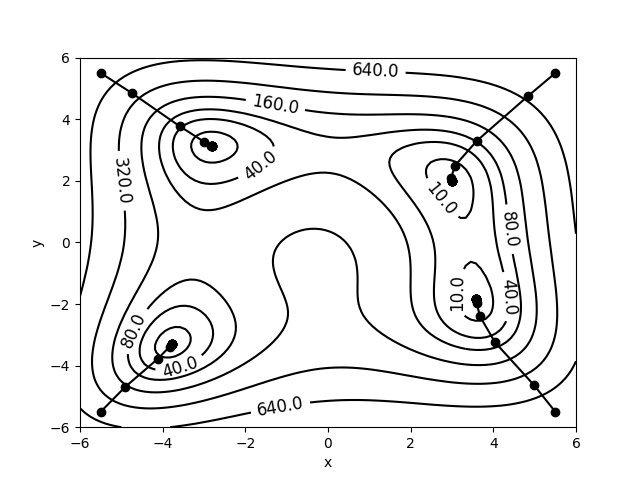
\includegraphics[scale=.8]{Figures/midtermExam_1}
        \end{center}
    \end{enumerate}

  \item % #3
    I used the following script to try and solve this problem.
    This script used the Cauchy Point method instead of the Dogleg because
    the Hessian is not always positive definite.
    \lstinputlisting[language=Python]{midtermExam_3.py}
    \lstinputlisting[language=Python]{cauchyPointMethod.py}

    The following image was output.
    \begin{center}
      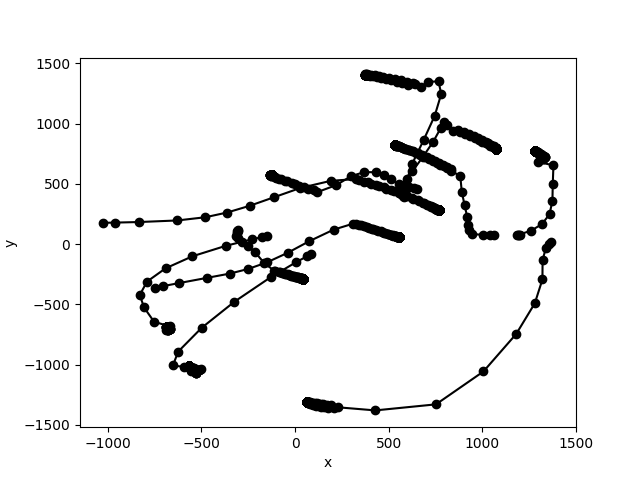
\includegraphics[scale=.8]{Figures/midtermExam_2}
    \end{center}

    My initial guess is described by the following vector.
    \begin{verbatim}
      array([ 1063.13361662,    74.46012024, -1028.17368688,   176.50472984,
          -307.20176908,   114.15633047,   653.7460869 ,   459.86440728,
          -149.77434281,    66.42794805,   595.42644861,   472.62825164,
          1201.24896009,    73.58942836,    86.98095451,   -83.02657181,
          1369.98306723,    17.08922723,   582.09891979,   392.28165874,
          -748.20081431,  -361.17194912]) 
    \end{verbatim}
    My final position was
    \begin{verbatim}
      array([  532.61219259,   821.19453455,   767.60659155,   280.21998863,
          44.6826028 ,  -289.15134043,  -125.32556221,   572.57935113,
        -685.19352323,  -684.78195294,   378.01600111,  1403.31655501,
        1280.25315662,   774.24900118,  -565.03254695, -1014.60503282,
          61.34327137, -1307.75659244,  1076.09321237,   791.56902424,
         554.21204466,    55.97004481])
    \end{verbatim}
    The value of my function was $7909452167.470356$.
    The method did not converge in 3000 steps.
    This seems pretty high, but I was unable to find a better solution.
    I believe that my final answer is pretty reasonable, and I think that
    maybe I can identify the different cities, but I am not very
    satisfied with this solution.
\end{enumerate}
\end{document}
